\section{Numerical Simulations}

\begin{frame}{Approximation of Coupled Shear Flow Problem}
\scriptsize
Consider
\begin{equation}
	\begin{split}
		&\partial_t Q(x,t) + \partial_x Q(x,t) =  D(w_x)Q(x,t)+ D_rEQ(x,t) \\
		&\partial_{t}w = \partial_{xx}w + \delta(\bar{\rho}-2\sqrt{\pi} c^0_0(x,t)).
	\end{split}
	\label{coupledsys_1d}
\end{equation}
\pause
\begin{table}[h]
	\centering
 \scalebox{0.95}{
		\begin{tabular}{|c|l|}
			\hline
			1. & $\frac{1}{2} \Delta t$ step on $\partial_t Q(x, t) = (D(w_x(x,t_n))+ D_rE)Q(x,t)$ \\
			2. & $\frac{1}{4} \Delta t$ step on $\partial_t w(x, t) = \delta(\bar{\rho} - 2\sqrt{\pi} c^0_0(x,t))$ \\
			3. & $\frac{1}{2} \Delta t$ step on $\partial_t w(x, t) = \partial_{xx} w(x, t)$ \\
			4. & $\frac{1}{4} \Delta t$ step on $\partial_t w(x, t) = \delta(\bar{\rho} -2\sqrt{\pi} c^0_0(x,t))$ \\
			5. & $\Delta t$ step on $\partial_t Q(x, t) + A \partial_x Q(x, t) = 0$ \\
			6. & $\frac{1}{4} \Delta t$ step on $\partial_t w(x, t) = \delta(\bar{\rho} - 2\sqrt{\pi} c^0_0(x,t))$ \\
			7. & $\frac{1}{2} \Delta t$ step on $\partial_t w(x, t) = \partial_{xx} w(x, t)$ \\
			8. & $\frac{1}{4} \Delta t$ step on $\partial_t w(x, t) = \delta(\bar{\rho} -2\sqrt{\pi} c^0_0(x,t))$ \\
			9. & $\frac{1}{2} \Delta t$ step on $\partial_t Q(x, t) = (D(w_x(x,t_{n+1}))+ D_rE)Q(x,t)$ \\
			\hline
		\end{tabular}
	}
	\caption{Splitting algorithm for solving the coupled shear flow problem (\cite{dahm2024numericaldiscretisationhyperbolicsystems})}
\end{table}
We use an ODE solver for $1.+9.$, LeVeque’s high resolution wave propagation algorithm for $5.$ and finite difference methods for the evolution of $w$.
\end{frame}


\begin{frame}
	\scriptsize
	\begin{figure}[H]
		\centering
		\begin{minipage}{0.4\textwidth}
			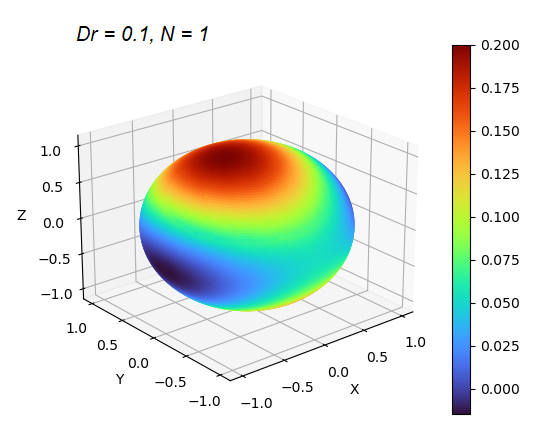
\includegraphics[scale=0.4]{Bilder_wx/wx=1_Dr=0.1_N=1}
		\end{minipage}
		\hfill 
		\begin{minipage}{0.4\textwidth}
			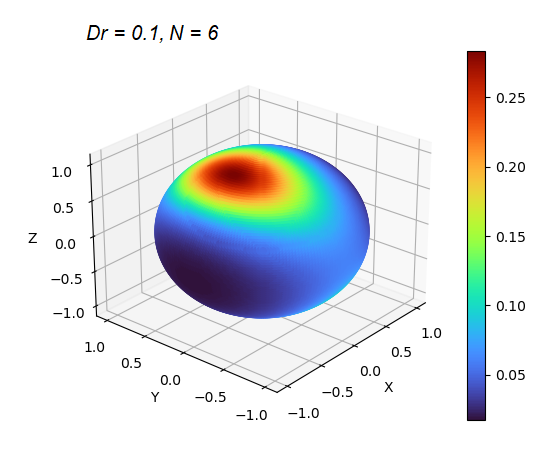
\includegraphics[scale=0.4]{Bilder_wx/wx=1_Dr=0.1_N=6}
		\end{minipage}
		\hfill 
		\begin{minipage}{0.4\textwidth}
			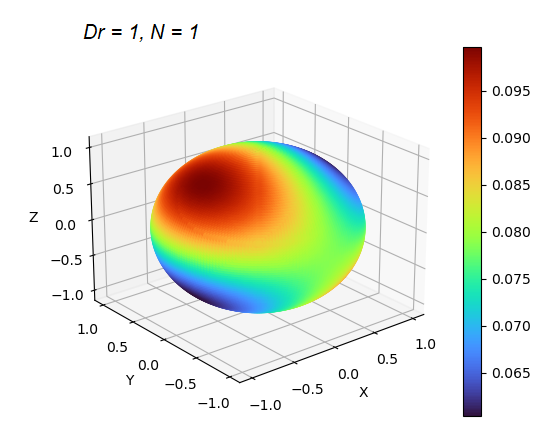
\includegraphics[scale=0.4]{Bilder_wx/wx=1_Dr=1_N=1}
		\end{minipage}
		\hfill 
		\begin{minipage}{0.4\textwidth}
			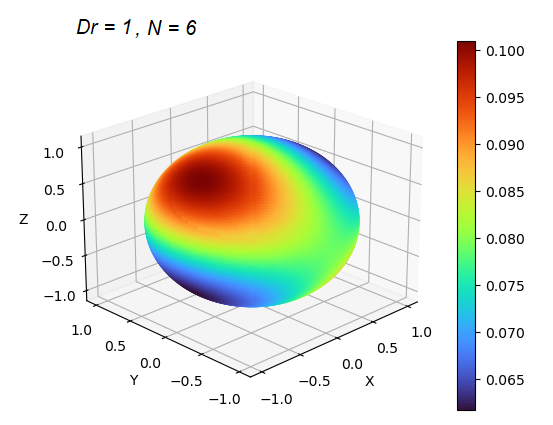
\includegraphics[scale=0.4]{Bilder_wx/wx=1_Dr=1_N=6}
		\end{minipage}
		\caption{ Numerical solution of the drift-diffusion term with constant externally imposed velocity gradient corresponding to shear flow using different values of $D_r$ and $N = 1,6$.}
	\end{figure}
\end{frame}
	

\begin{comment}
	Solve this problem by splitting it into two subproblems of the form
	\begin{enumerate}
		\item $\partial_t Q(x,t) + \textcolor{red}{A} Q_x=0$
		\item $\partial_t Q(x,t)  = \textcolor{blue}{\varphi} (Q(x,t))$
	\end{enumerate}
	\vspace{2mm}
Use finite volume methods for subproblem 1 and an ODE solver for subproblem 2.
\end{frame}
\end{comment}

\begin{comment}
\begin{frame}{Simulation of One-Dimensional Coupled Model}
	\scriptsize
	Consider the coupled moment system
	\begin{equation}
		\begin{split}
			&\partial_t Q(\boldsymbol{x},t) + \textcolor{red}{A}\partial_x Q(\boldsymbol{x},t) = \textcolor{blue}{\varphi} (Q(\boldsymbol{x},t)) \\
			&\partial_{t}w = \partial_{xx}w + \delta(\bar{\rho}-\rho(x,t)).
		\end{split}
		\label{coupledsys_1d}
	\end{equation}
	on the interval $[0, 100]$ with periodic boundary conditions and initial data
	\begin{align*}
		&c^0_0(x,0) = exp(-(x-50)^2)/(2 \cdot \sqrt{\pi}), \\
		&w(x,0) = 0 ,\\
		&D_r = 0.01, \delta = 1
	\end{align*}
\end{frame}
\end{comment}

\begin{comment}
\begin{frame}
	\scriptsize
	\begin{enumerate}
		\item Solve the drift diffusion equation
		\begin{equation*}
			\partial_t \left(\begin{array}{c}
				f_0 \\
				c_2^{-2} \\
				c_2^{-1} \\
				c_2^0 \\
				c_2^1 \\
				c_2^2
			\end{array}\right)  = \textcolor{blue}{\begin{pmatrix}
				0 & 0 & 0 & 0 & 0 & 0 \\
				0 & -6D_r & \frac{2}{7}w_x & 0 & 0 & 0 \\
				-\frac{\sqrt{15}}{5}w_x & -\frac{5}{7}w_x & -6D_r & \frac{3\sqrt{3}}{7}w_x & 0 & 0 \\
				0 & 0 & -\frac{4\sqrt{3}}{7}w_x & -6D_r & 0 & 0 \\
				0 & 0 & 0 & 0 & -6D_r & -\frac{5}{7} w_x\\
				0 & 0 & 0 & 0 & \frac{2}{7}w_x & -6D_r
			\end{pmatrix}} \cdot
			\left(\begin{array}{c}
				0 \\
				c^{-2}_2(t) \\
				c_2^{-1}(t) \\
				c_2^0(t) \\
				c_2^1(t) \\
				c_2^2(t)
			\end{array}\right).
		\end{equation*}
		with an implizit method.
		\item Solve 
		$$
		\partial_t \left(\begin{array}{c}
			f_0 \\
			c_2^{-2} \\
			c_2^{-1} \\
			c_2^0 \\
			c_2^1 \\
			c_2^2
		\end{array}\right) + \textcolor{red}{\begin{pmatrix}
			0 & 0 & \frac{\sqrt{15}}{15} & 0 & 0 & 0 \\
			0 & 0 & \frac{1}{7} & 0 & 0 & 0 \\
			\frac{\sqrt{15}}{15} & \frac{1}{7} & 0 & \frac{\sqrt{3}}{21} & 0 &  0 \\
			0 & 0 & \frac{\sqrt{3}}{21} & 0 & 0 & 0 \\
			0 & 0 & 0 & 0 & 0 & \frac{1}{7}\\
			0 & 0 & 0 & 0 & \frac{1}{7} & 0
		\end{pmatrix}} \partial_x \left(\begin{array}{c}
			f_0 \\
			c_2^{-2} \\
			c_2^{-1} \\
			c_2^0 \\
			c_2^1 \\
			c_2^2
		\end{array}\right) = 0
		$$
		with high resolution wave propagation algorithm.
	\end{enumerate}
\end{frame}
\end{comment}

\begin{comment}
\begin{frame}{Macroscopic Transport}
	\scriptsize
	Consider a Riemann Problem for externally imposed shear flow with $wx/D_r = 0.5$ for the left state and $wx/D_r = 1$ for the right state.
	\begin{figure}[H]
		\centering
		\begin{minipage}{0.32\textwidth}
			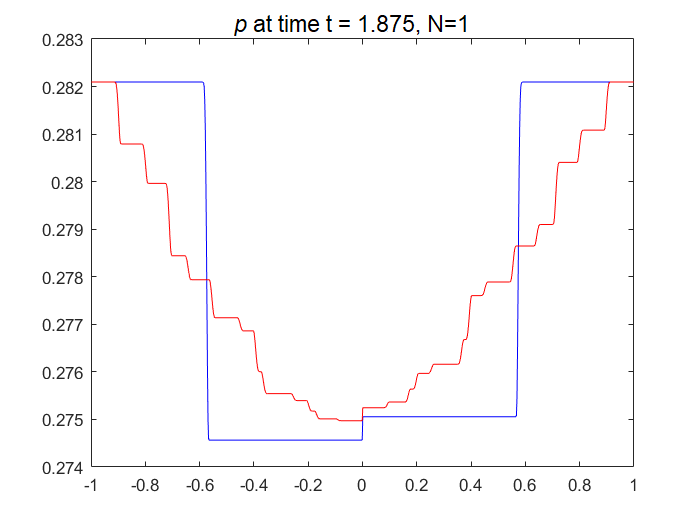
\includegraphics[width=\textwidth]{Bilder_wx/Wavepropa/red=12th_blue=2nd_wx=1_leftDr1_rightDr2_Awp12th}
		\end{minipage}
		\hfill
		\begin{minipage}{0.32\textwidth}
			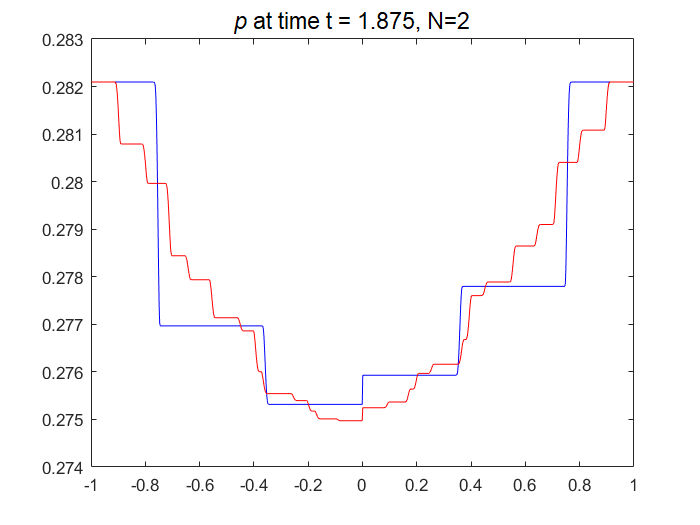
\includegraphics[width=\textwidth]{Bilder_wx/Wavepropa/red=12th_blue=4th_wx=1_leftDr1_rightDr2_Awp12th}
		\end{minipage}
		\hfill
		\begin{minipage}{0.32\textwidth}
			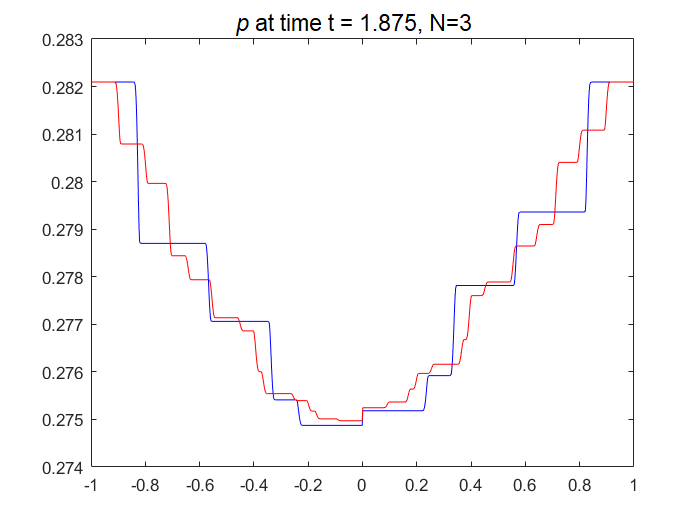
\includegraphics[width=\textwidth]{Bilder_wx/Wavepropa/red=12th_blue=6th_wx=1_leftDr1_rightDr2_Awp12th}
		\end{minipage}
		\vfill
		\begin{minipage}{0.32\textwidth}
			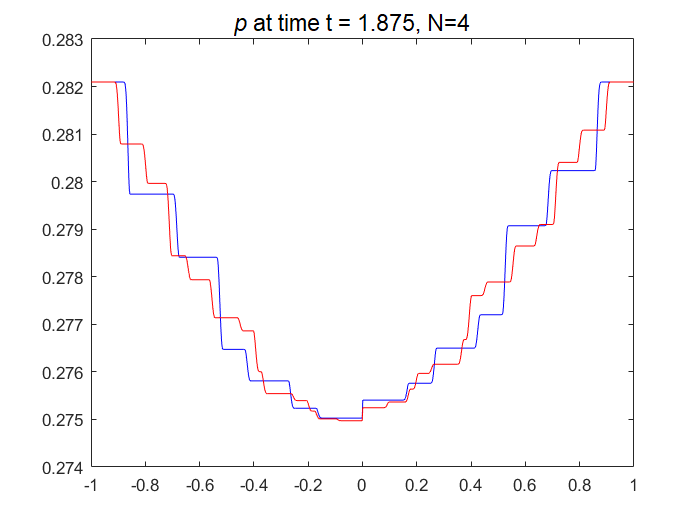
\includegraphics[width=\textwidth]{Bilder_wx/Wavepropa/red=12th_blue=8th_wx=1_leftDr1_rightDr2_Awp12th}
		\end{minipage}
		\hfill
		\begin{minipage}{0.32\textwidth}
			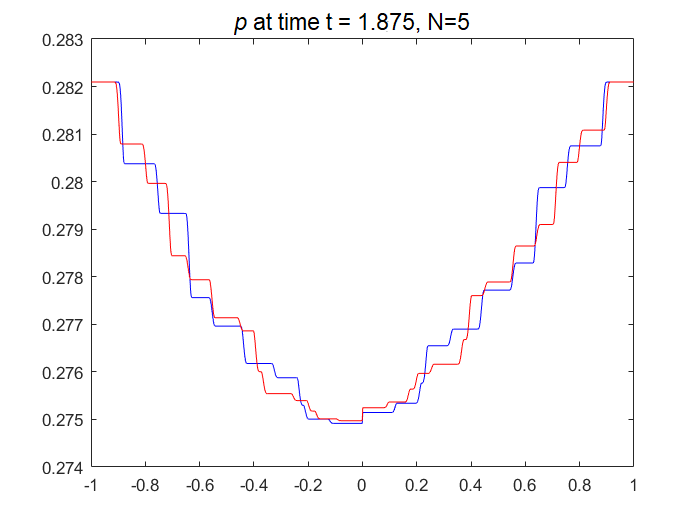
\includegraphics[width=\textwidth]{Bilder_wx/Wavepropa/red=12th_blue=10th_wx=1_leftDr1_rightDr2_Awp12th}
		\end{minipage}
		\hfill
		\begin{minipage}{0.3\textwidth}
			% Optional: Leave empty or add another image
		\end{minipage}
		\caption{Solution of the Riemann problem for $f_0$ at the time $t = 1.875$ using the moment system for different $N$ (blue curve) in comparison with $N = 6$ (red curve).}
	\end{figure}
\end{frame}
\end{comment}

\begin{comment}
\begin{frame}
	\scriptsize
	\textbf{Setting:}\\
	\begin{itemize}
		\item $w_{xi} = \pi \cdot \cos(\pi\cdot x_i)$
		\item Initial value $q(i,1)$ is set to $\frac{1}{2\sqrt{\pi}}$, rest $0$
		\item grid cells in x direction is set to $1000$
	\end{itemize}
	\begin{figure}[H]
		\centering
		\begin{minipage}{0.32\textwidth}
			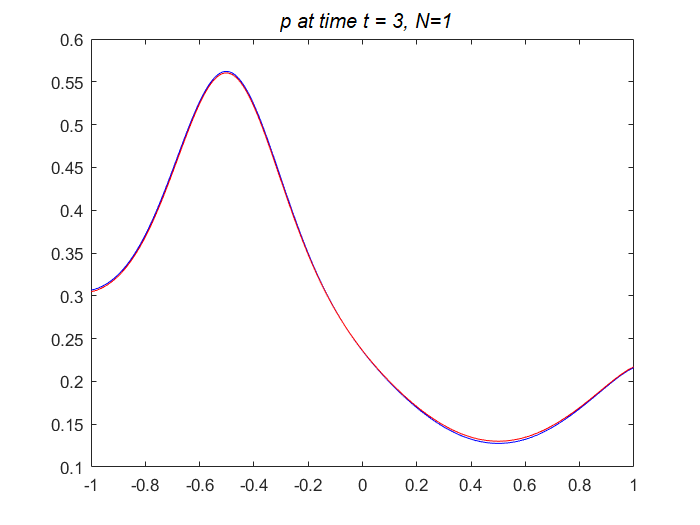
\includegraphics[width=\textwidth]{Bilder_wx/Wavepropa/red=12th_blue=2nd_wx=sin(pix)_Awp=0.5sqrt(pi)}
		\end{minipage}
		\hfill
		\begin{minipage}{0.32\textwidth}
			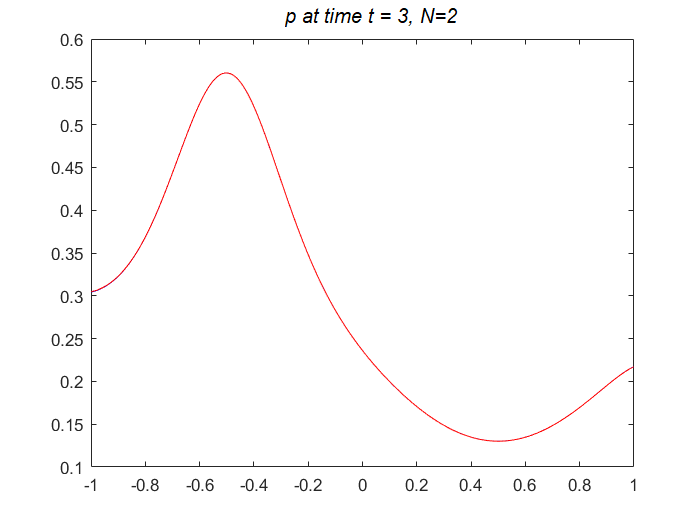
\includegraphics[width=\textwidth]{Bilder_wx/Wavepropa/red=12th_blue=4th_wx=sin(pix)_Awp=0.5sqrt(pi)}
		\end{minipage}
		\hfill
		\begin{minipage}{0.32\textwidth}
			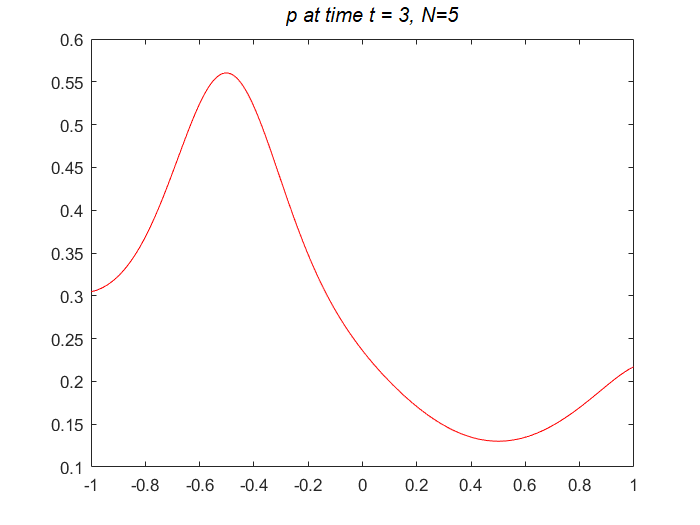
\includegraphics[width=\textwidth]{Bilder_wx/Wavepropa/red=12th_blue=10th_wx=sin(pix)_Awp=0.5sqrt(pi)}
		\end{minipage}
		\caption{Solution of the problem (\ref{conservationlaws}) for $f_0$ at the time $t = 3$ using the moment system for different $N$ (blue curve) in comparison with $N = 6$ (red curve).}
	\end{figure}
\end{frame}
\end{comment}



%%%%%%%%%%%% Case 1 %%%%%%%%%%%

\begin{frame}{Accuracy Study}
\scriptsize
Let  $c^0_0(x,0) = exp(-(x-50)^2)/(2 \cdot \sqrt{\pi})$ be the initial value.
\vspace{5mm}
\begin{table}[ht]
	\centering
	\begin{tabular}{|l|l|l|l|l|l|l|}
		\hline 
		& \multicolumn{2}{|c|}{$\mathrm{N}=1$} & \multicolumn{2}{|c|}{$\mathrm{N}=2$} & \multicolumn{2}{|c|}{$\mathrm{N}=3$} \\
		\hline 
		grid & $L1$-Error & EOC  & $L1$-Error & EOC  & $L1$-Error & EOC  \\
		\hline
		256 & $2.7197  \cdot 10^{-1}$ & & $1.9174\cdot 10^{-2}$&&$1.6585 \cdot 10^{-1}$&\\
		\hline
		512 & $1.0421 \cdot 10^{-1}$ &$1.38$ & $6.4197 \cdot 10^{-2}$&$1.57$&$ 5.4157 \cdot 10^{-2}$&$1.61$\\
		\hline 
		1024  &$3.0275 \cdot 10^{-2}$&$1.78$& $1.7984 \cdot 10^{-2}$&$1.83$&$ 1.5270 \cdot 10^{-2}$& $1.82$\\
		\hline
		2048 & $ 7.6037 \cdot 10^{-3}$ &$1.99$& $4.4721 \cdot 10^{-3}$&$2.0$&$3.6918 \cdot 10^{-3}$&$2.04$\\
		\hline
	\end{tabular}
	\caption{Accuracy study for the component $c^0_0$ of the coupled problem for shear flow using $D_r=1$. The reference solution, computed on a grid with $8192$ cells, uses the same number of moment equations as the coarse solution.  In all computations the time step was limited by a CFL condition with $cfl \leq 0.8$.}
	\label{tab:Dr=1_error_N=1,2,3vsN=1,2,3}
\end{table}
\end{frame}

%%%%%%%%%%%%%% Case 2, Dr=0.01 %%%%%%%%%%%%%%%%%

\begin{frame}{Accuracy Study}
	\scriptsize
	\begin{table}[H]
		\centering
		\begin{tabular}{|l|l|l|l|l|l|l|}
			\hline 
			& \multicolumn{2}{|c|}{$\mathrm{N}=1$} & \multicolumn{2}{|c|}{$\mathrm{N}=2$} & \multicolumn{2}{|c|}{$\mathrm{N}=3$}  \\
			\hline 
			grid & $L1$-Error & EOC  & $L1$-Error & EOC  & $L1$-Error & EOC\\
			\hline
			256  & $ 1.1624 \cdot 10^{-2}$ & & $ 2.6060\cdot 10^{-3}$&&$ 6.0421 \cdot 10^{-3}$& \\
			\hline
			512 & $ 1.2524 \cdot 10^{-2}$ & $-0.10$& $1.1655  \cdot 10^{-3}$&$1.16$& $ 1.1655 \cdot 10^{-3}$& $2.37$ \\
			\hline 
			1024  &$ 1.3168 \cdot 10^{-2}$&$-0.07$& $3.1649 \cdot 10^{-3}$& $-1.44$ & $8.0673\cdot 10^{-4}$&$0.53$\\
			\hline
			2048 & $ 1.3310 \cdot 10^{-2}$ &$-0.01$& $  3.4125 \cdot 10^{-3}$&$-0.10$& $ 5.5722 \cdot 10^{-4}$&$0.53$\\
			\hline
		\end{tabular}
		\caption{Accuracy analysis for the component $c^0_0$ of the coupled problem for shear flow using $D_r=0.01$. The reference solution, computed on a grid with $8192$ cells using $N=6$. In all computations the time step was limited by a CFL condition with $cfl \leq 0.8$.}
		\label{tab:Dr=0.01_error_N=1,2,3vsN=6}
	\end{table}
\end{frame}


\begin{frame}{Accuracy Study}
	\scriptsize
	\begin{table}[H]
		\centering
		\begin{tabular}{|l|l|l|l|l|}
			\hline 
			& \multicolumn{2}{|c|}{$\mathrm{N}=4$} & \multicolumn{2}{|c|}{$\mathrm{N}=5$}   \\
			\hline 
			grid & $L1$-Error & EOC  & $L1$-Error & EOC  \\
			\hline
			256  & $5.9343\cdot 10^{-3}$ & & $ 6.2261\cdot 10^{-3}$& \\
			\hline
			512 & $ 2.1285 \cdot 10^{-3}$ & $1.47$ & $2.3204  \cdot 10^{-3}$&$1.42$ \\
			\hline 
			1024  &$ 6.1323\cdot 10^{-4}$&$1.79$& $ 6.8919 \cdot 10^{-4}$& $1.75$ \\
			\hline
			2048 & $ 2.4303 \cdot 10^{-4}$ &$1.33$& $ 1.7118 \cdot 10^{-4}$&$2.0$\\
			\hline
		\end{tabular}
		\caption{Accuracy analysis for the component $c^0_0$ of the coupled problem for shear flow using $D_r=0.01$. The reference solution, computed on a grid with $8192$ cells using $N=6$. In all computations the time step was limited by a CFL condition with $cfl \leq 0.8$.}
		\label{tab:Dr=0.01_error_N=4,5vsN=6}
	\end{table}
\end{frame}


%%%%%%%%% Case 2, Dr = 0.05 %%%%%%%%%%%%%%%

\begin{frame}{Accuracy Study}
	\scriptsize
	\begin{table}[H]
		\centering
		\begin{tabular}{|l|l|l|l|l|l|l|}
			\hline 
			& \multicolumn{2}{|c|}{$\mathrm{N}=1$} & \multicolumn{2}{|c|}{$\mathrm{N}=2$} & \multicolumn{2}{|c|}{$\mathrm{N}=3$}  \\
			\hline 
			grid & $L1$-Error & EOC  & $L1$-Error & EOC  & $L1$-Error & EOC\\
			\hline
			256  & $ 1.4093 \cdot 10^{-2}$ & & $ 8.4036 \cdot 10^{-3}$&&$6.6520  \cdot 10^{-3}$& \\
			\hline
			512 & $3.4409 \cdot 10^{-3}$ & $2.03$& $ 2.0240  \cdot 10^{-3}$&$2.05$& $ 2.0034 \cdot 10^{-3}$&$1.73$ \\
			\hline 
			1024  &$ 1.5602\cdot 10^{-3}$&$1.14$& $ 4.3070 \cdot 10^{-4}$&$2.23$ & $5.4486\cdot 10^{-4}$&$1.87$\\
			\hline
			2048 & $1.4673\cdot 10^{-3}$ &$0.08$& $ 1.2731 \cdot 10^{-4}$&$1.75$& $ 1.3623 \cdot 10^{-4}$&$1.99$\\
			\hline
		\end{tabular}
		\caption{Accuracy analysis for the component $c^0_0$ of the coupled problem for shear flow using $D_r=0.05$. The reference solution, computed on a grid with $8192$ cells using $N=6$. In all computations the time step was limited by a CFL condition with $cfl \leq 0.8$.}
		\label{tab:Dr=0.05_error_N=1,2,3vsN=6}
	\end{table}
\end{frame}


%%%%%%%%%%%%%%% Case 2, Dr=1 %%%%%%%%%%%%%%

\begin{frame}{Accuracy Study}
	\scriptsize
	\begin{table}[H]
		\centering
		\begin{tabular}{|l|l|l|l|l|l|l|}
			\hline 
			& \multicolumn{2}{|c|}{$\mathrm{N}=1$} & \multicolumn{2}{|c|}{$\mathrm{N}=2$} & \multicolumn{2}{|c|}{$\mathrm{N}=3$}  \\
			\hline 
			grid & $L1$-Error & EOC  & $L1$-Error & EOC  & $L1$-Error & EOC\\
			\hline
			256  & $  2.7228  \cdot 10^{-1}$ & & $ 1.9183 \cdot 10^{-1}$&&$1.6589 \cdot 10^{-1}$& \\
			\hline
			512 & $1.0452 \cdot 10^{-1}$ &$1.38$ & $ 3.1259 \cdot 10^{-2}$&$2.61$& $ 5.4197 \cdot 10^{-2}$&$1.61$\\
			\hline 
			1024  &$3.0596 \cdot 10^{-2}$&$1.77$& $1.8077 \cdot 10^{-2}$&$0.79$ & $1.5310\cdot 10^{-2}$&$1.82$\\
			\hline
			2048 & $ 7.9252\cdot 10^{-3}$ &$1.94$& $ 4.5655\cdot 10^{-3}$&$1.98$& $3.7315  \cdot 10^{-3}$&$2.03$\\
			\hline
		\end{tabular}
		\caption{Accuracy analysis for the component $c^0_0$ of the coupled problem for shear flow using $D_r=1$. The reference solution, computed on a grid with $8192$ cells using $N=6$. All simulations employed a time step constrained by a CFL condition with $cfl \leq 0.8$.}
		\label{tab:Dr=1_error_N=1,2,3vsN=6}
	\end{table}
\end{frame}


\begin{frame}{Cluster Formation}
	\scriptsize
	Let 
	\begin{align*}
		c^0_0 (x,0) = (1+(1\cdot10^{-4} \cdot \eta(x)-5\cdot10^{-5}))/(2\sqrt{\pi}),
	\end{align*}
where $\eta(x)$ is a random variable taking values in the interval $\pm \frac{1}{2}$.
	
	\begin{figure}
		\centering
		\begin{minipage}{0.46\textwidth}
			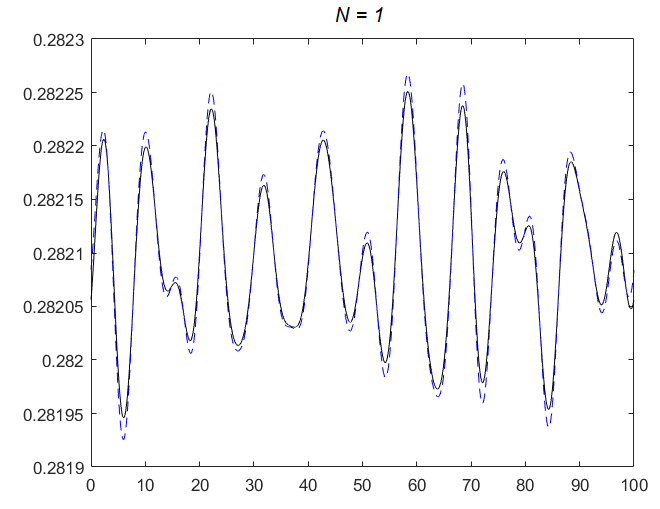
\includegraphics[width=\textwidth]{Bilder_wx/ClusterFormation/N=1vsN=6_Dr=0.05_mx=8192}
		\end{minipage}
		\hfill
		\begin{minipage}{0.46\textwidth}
			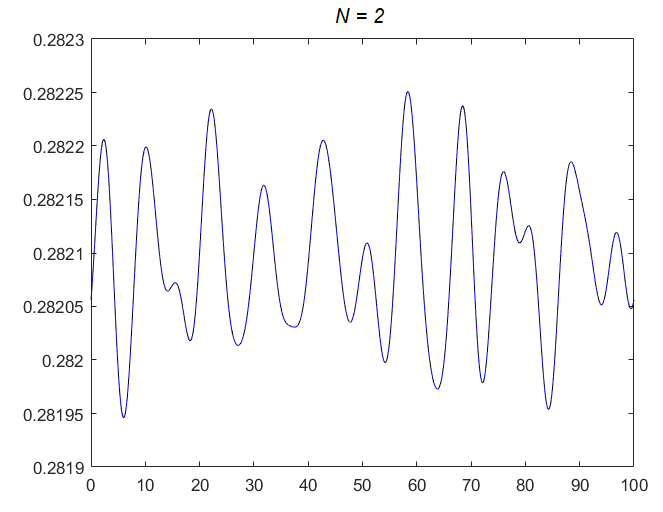
\includegraphics[width=\textwidth]{Bilder_wx/ClusterFormation/N=2vsN=6_Dr=0.05_mx=8192}
		\end{minipage}
		\caption{Approximation of the coupled problem for shear flow with $D_r =0.05$. The plot shows the density at time $t=30$ for $N = 1$ and $N = 2$ (blue line). A reference solution is calculated with $N = 6$ moment equations (black line).}
		\label{ClusterFormation}
	\end{figure}
	%The Figure (\ref{ClusterFormation}) shows that using $N = 1$ moment equations, compared to the reference solution with $N = 6$, already provides a good approximation of cluster formation. The numerical solution for $N=2$ aligns very well with the reference solution.
\end{frame}

\begin{comment}
\begin{frame}
		\begin{figure}
		\centering
		\begin{minipage}{0.46\textwidth}
			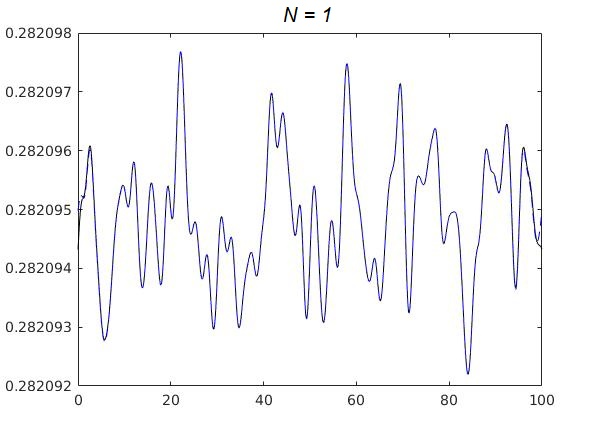
\includegraphics[width=\textwidth]{Bilder_wx/ClusterFormation/cluster_N=1vsN=6_Dr=1_mx=8192}
		\end{minipage}
		\hfill
		\begin{minipage}{0.46\textwidth}
			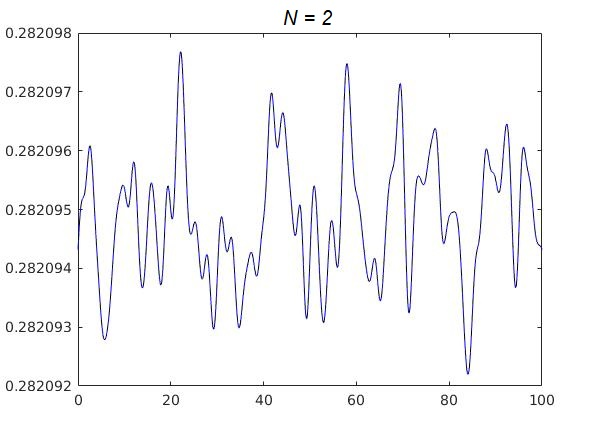
\includegraphics[width=\textwidth]{Bilder_wx/ClusterFormation/cluster_N=2vsN=6_Dr=1_mx=8192}
		\end{minipage}
		\caption{Approximation of the coupled problem for shear flow with $D_r =1$. The plot shows the density at time $t=30$ for $N = 1$ and $N = 2$ (blue line). The black line represents a reference solution calculated with $N = 6$ moment equations.}
		\label{ClusterFormation_Dr=1}
	\end{figure}
\end{frame}
\end{comment}


\begin{comment}
\begin{frame}
	\begin{figure}
		\centering
		\begin{minipage}{0.32\textwidth}
			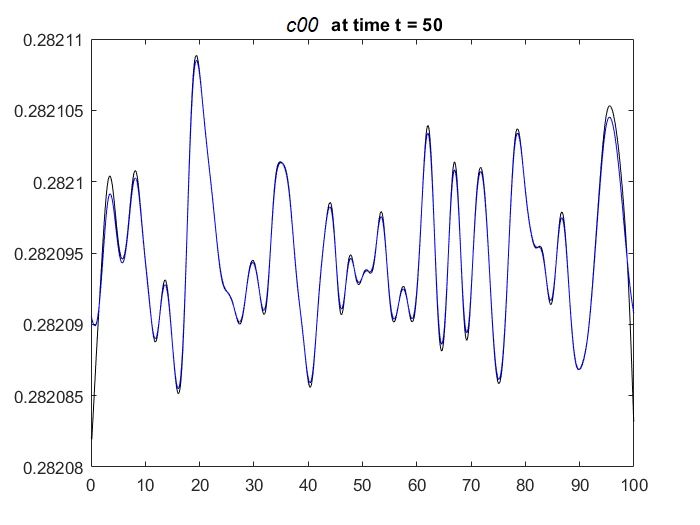
\includegraphics[width=\textwidth]{Bilder_wx/ClusterFormation/N=1vsN=6_t=50}
		\end{minipage}
		\hfill
		\begin{minipage}{0.32\textwidth}
			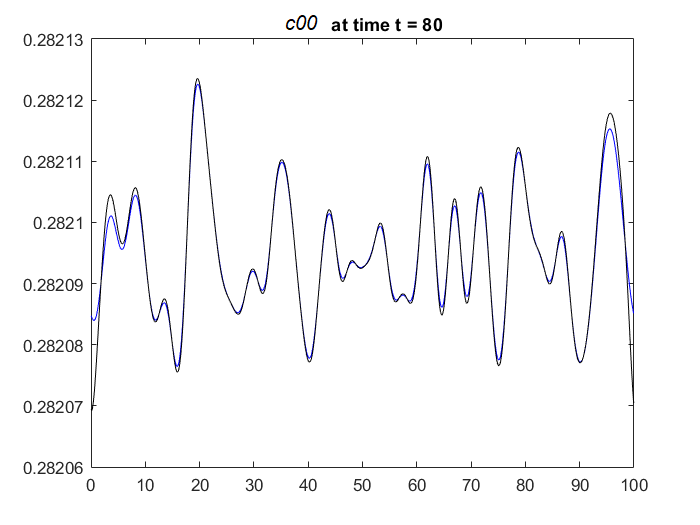
\includegraphics[width=\textwidth]{Bilder_wx/ClusterFormation/N=1vsN=6_t=80}
		\end{minipage}
		\hfill
	\begin{minipage}{0.32\textwidth}
		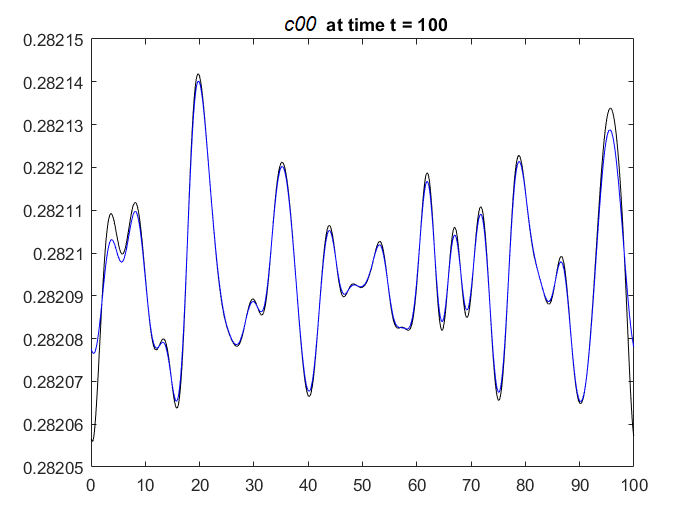
\includegraphics[width=\textwidth]{Bilder_wx/ClusterFormation/N=1vsN=6_t=100}
	\end{minipage}
		\caption{Numerical simulation of cluster formation for density at different times with $N = 1$ (blue) and $N = 6$ (black). All computations used 1024 grid cells.}
		\label{ClusterFormation_time_Dr=1}
	\end{figure}
\end{frame}
\end{comment}

